\chapter{Narrative planning}
\label{ch:planning}
\textit{This chapter will discuss the use of a narrative planner as used by many of my sources. I want to incorporate a narrative planner that smartly uses \diage to manipulate a narrative and conveys that in a way we petty humans can understand}
\\\\
A lot of related work as gone into the use of a planning system that decides on the narrative structure. Researchers like Riedl and Young~\cite{Riedl03character-focusednarrative}\cite{Riedl:2003:MIU:860575.860694}\cite{Riedl:2004:IPM:1018409.1018753} and Cavazza~\cite{Cavazza:2002:CIS:630325.630747} have been researching the use of artificial intelligence for years, and have made some interesting planning systems like \textit{Memesis}~\cite{young2003towards}. To help me answer my questions, I have developed my own narrative planner that tracks and generates plot points that the player can resolve to further the characters story.

\section{Events}
Riedl and Young\cite{Riedl:2004:IPM:1018409.1018753} and Julie Porteous and Marc Cavazza\cite{Porteous:2009:CNG:1695522.1695557} have demonstrated that stories are perfectly suited to be represented as a sequence of temporal and causal events. Porteous and Cavazza suggest to use events as a constraint for partial temporal order. Defining operators as the following:\\\\
\begin{tabular}{|l||l|}
\hline 
operator & meaning \\ 
\hline
\hline 
\textit{sometime-before a b} & \textit{b} must be made true for the first time before \textit{a} \\ 
\hline 
\textit{sometime a} & predicate \textit{a} must be true at some stage of the narrative \\ 
\hline 
\textit{at-end a} & predicate \textit{a} must be true at the end of the narrative \\ 
\hline 
\end{tabular} 
\\\\
These operators ensure that we have some control and gives us a partial temporal order, partial because not all of the events are ordered with respect to each other. The table is further expanded upon in their paper \textit{Controlling Narrative Generation with Planning Trajectories: the Role of Constraints}~\cite{Porteous:2009:CNG:1695522.1695557}.

The \diage planner uses event constraints like this to layer plots and direct the player on what to do next. In the context of a \rogue we don't know when the story is going to stop, as it stops with the death of the player character. That could be within 2 minutes, but it could be several weeks. \diage takes this into account by keep adding segments onto a story, sometimes using information gained from previous plots and at other times creating entire new spaces and NPCs therein. So the operators that Porteous uses we use within these small story steps instead of the entire narrative. \diage tells us the story of the player character and how \he influenced the world around him.

\section{Initial Generation}
Depending on the input given and the desires of the developer, \diage does the initial generation of the game world and plots in varying degrees, as seen in algorithm~\ref{alg:initial_setup}. If no input is given at all, \diage will just generate a random amount of entities to populate the world. Input can be given either within the game code, or with a DML file (further discussed in the next chapter). Whether specified or not, the player character needs a initial constraint. This constraint is \his first 'objective'. This initial constraint can be given within the input, otherwise \diage will take an entity within the world and sets that as player constraint. With in the algorithm we see a section dedicated to custom rules. These rules can manipulate anything within the story setting. As an example I created a rule that randomly sets entities to a space. The given example is purely non-deterministic, but is a simple matter to populate the spaces more evenly with the entities. This rule system is used throughout \diage as a generalized form to give the developer more control on what a given entity can do.

\begin{algorithm}
	\KwIn{entities; customRules;}
	\KwOut{Initial world state}
	let \textit{entities} be all entities within current world state\;
	let \textit{customRules} be the custom behaviour as specified by the developer\;
	\ForEach{rule in customRules}{
		rule.Invoke();
	}
	\If{entities.count $\leq$ 0}{
		entities = GenerateRandomEntities(\textit{max})\;
	}
	\If{player.constraint == null}{
		\textbf{select random} \textit{e} \textbf{from} \textit{entities}\;
		player.constraint = \textit{e}\;
	}
    \caption{Initial planning}\label{alg:initial_setup}
\end{algorithm}
\begin{procedure}
	\tcc{Populates the spaces with the current entities within world state}
	\KwIn{entities; spaces;}
	\KwOut{All entities are randomly moved to a space}
	let \textit{entities} be all objects within current world state, excluding spaces\;
	let \textit{spaces} be all spaces within current world state\;
	\While{entities.count $>$ 0}{
		\textbf{select random} \textit{s} \textbf{from} \textit{spaces}\;
		entities.pop().MoveToSpace(s)\;
	}
	\caption{PopulateSpaces()}\label{proc:rule_example}
\end{procedure}

\section{Step Generation}
When the initial generation is complete, the player should carry out \his objective. When the objective has been completed, the planner will automatically start a step generation\footnote{in want of a better word. The term \textit{step} comes from cellular automata, which I'm currently working on}. This generation is like the initial generation but uses the actor attribute system and the player as extra input. The attribute system will be covered in a later section. This step generation looks at all the given variables and generates a new constraint for the player(see procedure~\ref{proc:generate_constraint}). The longer the character's life, the more exact this generation will be. For any action taken by the player can be used in the generation. It must be said that the actions that the planner can take needs to be specified by the author. 
\begin{algorithm}
	\KwIn{entities; actors; player; customRules;}
	\KwOut{new world state}
	let \textit{entities} be all entities, excluding actors and the player\;
	let \textit{actors} be all actors, including the player\;
	\ForEach{actor in actors}{
		actor.rules.Invoke()\;
	}
	\tcc{It's possible that one of the rules gave the player a constraint, so we'll check}
	\If{player.constraint == null}{
		GenerateConstraint(player)\;
	}
	\ForEach{rule in customRules}{
		rule.Invoke()\;
	}
	\caption{Step planning}\label{alg:step_planning}
\end{algorithm}
\begin{procedure}
	\KwIn{player}
	\KwOut{new constraint for the player}
		\eIf{rules.count $\geq$ 0}{
			\ForEach{item in rules}{
				rules.invoke(player)\;
			}}{
				\textbf{select random} \textit{e} \textbf{from} \textit{entities}\;
				player.constraint = \textit{e}\;
			}
	\caption{GenerateConstraint(Player)}\label{proc:generate_constraint}
\end{procedure}
\section{Planning flow}
The previous sections described the processes that \diage goes through when generating a new world. The flowchart in figure~\ref{fig:diage_flowchart} displays the steps taken by the planner. The initial generation influences the world by setting up spaces, actors, and objects and manipulating these entities by their specific rules. After this, the player can, and will, influence the world by acting in it. The planner keeps track of \his actions and saves this for future story generation \footnote{For example; a foe thought defeated returns for a rematch.}. The step generation gets activated automatically when the player's constraint is removed, i.e. a plot is resolved. This can also be manually activated by the author on whatever occasion or event \he wishes. After the step generation the player gets \his new constraint and, depending on the generative rules used, the world can be manipulated too. Be that actors that move, or new spaces that are generated. The step generation is highly dependant upon the player's attributes, as everything can react to the gain or loss between story steps\footnote{Mental note: one of the papers referenced this as a beat, might be a good idea!}. The actor attributes are a powerful tool in the \diage arsenal, and the (game)world literary revolves around them.
It has to be noted, that the design of \diage works with semi-persistent worlds too. The world data can be saved to be used in a later play-through, giving the world a whole epic of one player, and starting the next. 
\begin{figure}[p]
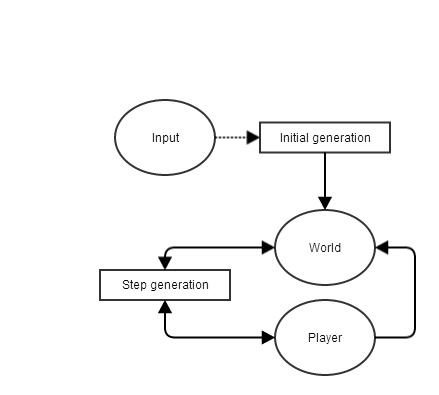
\includegraphics[scale=.8]{diage_planner}
\caption{Diage Planner flowchart}\label{fig:diage_flowchart}
\end{figure}

\section{Actor attributes}
All actor entities have a attribute system in place that give them unique skills or personalities. These attributes can interact with the planner to create different outcomes of the step generation. The attributes can also communicate directly with a player. For example; the player could have a attribute \textit{Archery} where an actor in the role of shop keeper might offer the player a exceptional bow if said attribute is above a value of 50. Even if we put it less 'gamey' and more in a narrative setting, we could add personality archetypes (sometimes called alignments in RPGs) as a attribute. For example; the \textit{Lawful Good} archetype will be friendly to all other on the \textit{Good} axis, but completely antagonistic towards any on the \textit{Chaos} side (see figure~\ref{fig:dnd} for reference).
The attribute system can create a wide variety of emergent behaviour and will be expanded upon in a following chapter~\citationneeded
\begin{figure}[p]
	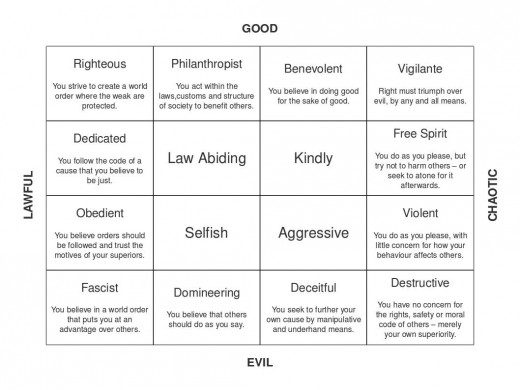
\includegraphics[scale=.8]{alignment}
	\caption{\textit{Dungeons \& Dragons} alignment sheet}\label{fig:dnd}
\end{figure}